\documentclass{article} % For LaTeX2e
\usepackage{iclr2026_conference,times}

% Optional math commands from https://github.com/goodfeli/dlbook_notation.
\input{math_commands.tex}

\usepackage{hyperref}
\usepackage{url}
\usepackage{graphicx}
\usepackage{float}
\title{SCORE: Tokenization-Aware Transformer for Symbolic Music Generation with Expressions}

% Authors must not appear in the submitted version. They should be hidden
% as long as the \iclrfinalcopy macro remains commented out below.
% Non-anonymous submissions will be rejected without review.

\author{Vishakh.~Begari \thanks{https://orcid.org/0009-0008-9399-8581} \\
Independent Researcher\\
Bavaria, Germany \\
\texttt{vibedjentle@gmail.com}
}

% The \author macro works with any number of authors. There are two commands
% used to separate the names and addresses of multiple authors: \And and \AND.
%
% Using \And between authors leaves it to \LaTeX{} to determine where to break
% the lines. Using \AND forces a linebreak at that point. So, if \LaTeX{}
% puts 3 of 4 authors names on the first line, and the last on the second
% line, try using \AND instead of \And before the third author name.

\newcommand{\fix}{\marginpar{FIX}}
\newcommand{\new}{\marginpar{NEW}}

\iclrfinalcopy % Uncomment for camera-ready version, but NOT for submission.
\begin{document}

\maketitle

\begin{abstract}
Ever since the electrification of guitar, there has been an explosion in rhythmic complexity,
tone experimentation and playing techniques. In this paper, a novel tokenisation method is proposed,
which encapsulates the various guitar techniques and a sequence level attention component 
for the transformer architecture, 
which captures segmentation between musical phrases. The given approach enables 
efficient batching of variable length musical phrases while preserving their contextual coherence.
\end{abstract}

\section{Introduction}\label{sec1}

A \textit{riff} is a short, repeated motif or figure in the melody or accompaniment of a 
musical composition \citep{randel86}. This type of composition is particularly prevalent 
in rock, metal, blues, funk and jazz. It is often the main feature that gives character 
and structure to a song. Developments in Transformers architecture have inspired 
many to generate sequences by treating musical notes as symbolic language
\citep{Vaswani2}
\citep{10.1145/3394171.3413671}
\citep{wu2020jazz}
\citep{ens2020mmm}
\citep{symbolic}
\citep{yu2022museformer}. 
\citep{dong2023multitrack}
\citep{app13074543}
\citep{agostinelli2023musiclmgeneratingmusictext} 
\citep{copet2024simplecontrollablemusicgeneration} 
\citep{doi:10.1177/14727978251337904}.
Generating modern music demands capturing not only note patterns but also the associated expressions. 

A widely adopted method for representing musical notes digitally is the MIDI format \citep{craig2025midifileformat}, 
which encodes pitch, duration, and dynamics. Using such a format for musical expression has limitations like resolution 
and bandwidth constraints \citep{midi_short} when compared to richer representations like 
audio recordings and detailed scores. Modern guitar riffs frequently employ intense and abrupt expressive
techniques, which contribute significantly to its overall identity \citep{vallejo2021development}. To accurately represent the nuanced 
expressive elements of modern music, a score based format is preferable over simpler encodings like MIDI.
The proposed method requires a tokenisation scheme that represents notes, beats, beat types and their associated accents, 
necessitating a dataset that includes expressive performance details.

In the context of symbolic music, notes are represented as sequences of discrete tokens. This requires a tokenisation scheme which directly affects how effectively a 
model can learn and generate coherent musical structures. Most existing approaches rely on methods similar to text 
processing such as BPE (Byte Pair Encoding) \citep{sennrich2016neuralmachinetranslationrare}, WordPiece \citep{sentencepiece}
and SentencePiece \citep{kudo2018sentencepiecesimplelanguageindependent}. Although subword tokenization improves 
the structure \citep{kumar2023wordsmusicstudysubword} \citep{bpe-symbolic-music},
it becomes limited when dealing with the expressive element combinations of modern music. Recent studies 
\citep{gardin2024musiclang} have explored modeling chords based on scale degree, tonality and octave, and 
notes encoded relative to the current chord. This approach, however, is unable to produce every possible chord, 
particularly when dissonance is involved, which is becoming increasingly popular in modern metal. 
Most prior studies use absolute pitch values \citep{awsdeepcomposer}, some \citep{kermarec2022tokenization} investigate the use of pitch intervals.
This introduces an additional processing step, increasing inference time. Another common strategy treats each 
unique chord as a separate token, resulting in a large vocabulary that may include thousands of tokens 
representing all possible chords in the dataset \citep{harmony} \citep{Chordinator}. 
\citet{chen2020automatic} proposes a pre-defined set of rhythmic groove patterns. This limits the model's ability to generate novel rhythms. 

Despite the growing body of work on symbolic music generation, there is little to no prior work 
specifically addressing expressive guitar music that captures techniques such as bends, slides, 
and chords in a tokenized representation. To address these limitations, a tokenisation scheme is proposed, that captures single and multiple musical notes efficiently and 
their associated accentuated elements. Furthermore, a sequence level attention mechanism is introduced to capture the segmentation
between different musical phrases, facilitating batching of variable length phrases while maintaining musical context.
The modified architecture is trained and evaluated on a dataset \citep{SCORESET} that includes guitar specific techniques.

While direct comparison with existing methods is not feasible due to differences in 
model compatibility and expressive feature representation, the proposed method is 
evaluated using quantitative metrics. The model is trained to minimize KL 
divergence across pitch, beat, beat type, and expression similarity. The source code of this work is available at \url{https://github.com/DjentleViBe/SCORE}.

\section{Methods}\label{sec:proposedmethod}

\subsection{Tokenisation}\label{sec:tokenisation}
\subsubsection{Note representation}\label{sec:note}


\begin{table}[t]
\centering
\begin{minipage}{0.48\linewidth}
\centering
\caption{Beat type. $d$ = 7 for dotted note, 0 otherwise.}
\label{tab:bt}
\begin{center}
  \begin{tabular}{ll}
    \multicolumn{1}{c}{\bfseries $b_{t}$}  &\multicolumn{1}{c}{\bfseries Value}
  \\ \hline \\
  Triplet(3)        & 1 + $d$          \\
  Quintuplet(5)     & 2 + $d$          \\
  Sextuplet(6)      & 3 + $d$          \\
  Septuplet(7)      & 4 + $d$          \\
  Nonuplet(9)       & 5 + $d$          \\
  Undecuplet(11)    & 6 + $d$          \\
  \end{tabular}
  \end{center}
\end{minipage}\hfill
\begin{minipage}{0.48\linewidth}
\centering
\caption{Beats.}
\label{tab:duration}
\begin{center}
  \begin{tabular}{ll}
    \multicolumn{1}{c}{\bfseries $b_{b}$}  &\multicolumn{1}{c}{\bfseries Value}
   \\ \hline \\
  1 / 64  & 0          \\
  1 / 32  & 1          \\
  1 / 16  & 2          \\
  1 / 8  & 3          \\
  1 / 4  & 4          \\
  1 / 2  & 5          \\
  1 & 6          \\
  \end{tabular}
  \end{center}
\end{minipage}
\end{table}
In place of absolute pitch indices, both fret and string numbers are employed to represent notes.  This approach allows for a more compact representation of notes, 
as the same pitch can be played on different strings and frets. This is particularly relevant to guitar music, where notes can be produced at multiple 
fretboard positions, often resembling chord shapes. The model focuses on learning the relative motion of notes across frets, emphasizing positional 
changes rather than absolute pitch representation. This provides flexibility to accommodate alternative
tunings \citep{Weissman2006GuitarTunings}. The formula for note encodings for fretted string instrument is given by: 
\begin{align}
n_e = n_i + 2b_t \cdot n_s \cdot n_{ps} + 2b_b \cdot n_s \cdot n_{ps}
\end{align}
where, $n_s$ = number of strings, $n_{ps}$ = number of pitch steps per string.
\begin{align}
n_i = f_n + s_n \cdot n_{ps} + n_s \cdot n_{ps} \cdot n_{val}
\end{align}
where, $f_n$ = fret number, $s_n$ = string number and $n_{val}$ = 1 for palm mute, 0 otherwise; $b_t$ and $b_b$ are defined in ~\ref{tab:bt} and ~\ref{tab:duration} respectively.

\subsubsection{Accent representation}
A description of expressive elements is provided in ~\citep{begari2025scoresetdatasetguitarprofiles}.
An accent token is appended to the note token from Section~\ref{sec:note} to indicate the presence of an expressive element. 
For chords, the accent token is added before the next consecutive note token.
A C major chord as shown in Figure~\ref{fig:chord} comprises of 3 notes - root note (C) played on the 
fret 2, 5th string , major third (G) on fret 1, 4th string and perfect fifth (E) on 
fret 2, 1st string \citep{Alexander2019GuitarChordsInContext}. The tokenization for the chord is as follows:
\texttt{15413, 27051, 15389, 27051, 15321, 27051}. Here, \texttt{27051} is the chord accent token, BARRE\_NOTE\textsuperscript{~\ref{app:secA1}}. Similarly, for a bend note
depicted in Figure~\ref{fig:bend}, the tokenization is: \texttt{15461, 27052}. Here, \texttt{27052} is the bend accent token, BEND\_NOTE\_1\textsuperscript{~\ref{app:secA1}}.
\begin{figure}[t]
\centering
\begin{minipage}{0.48\linewidth}
  \centering
  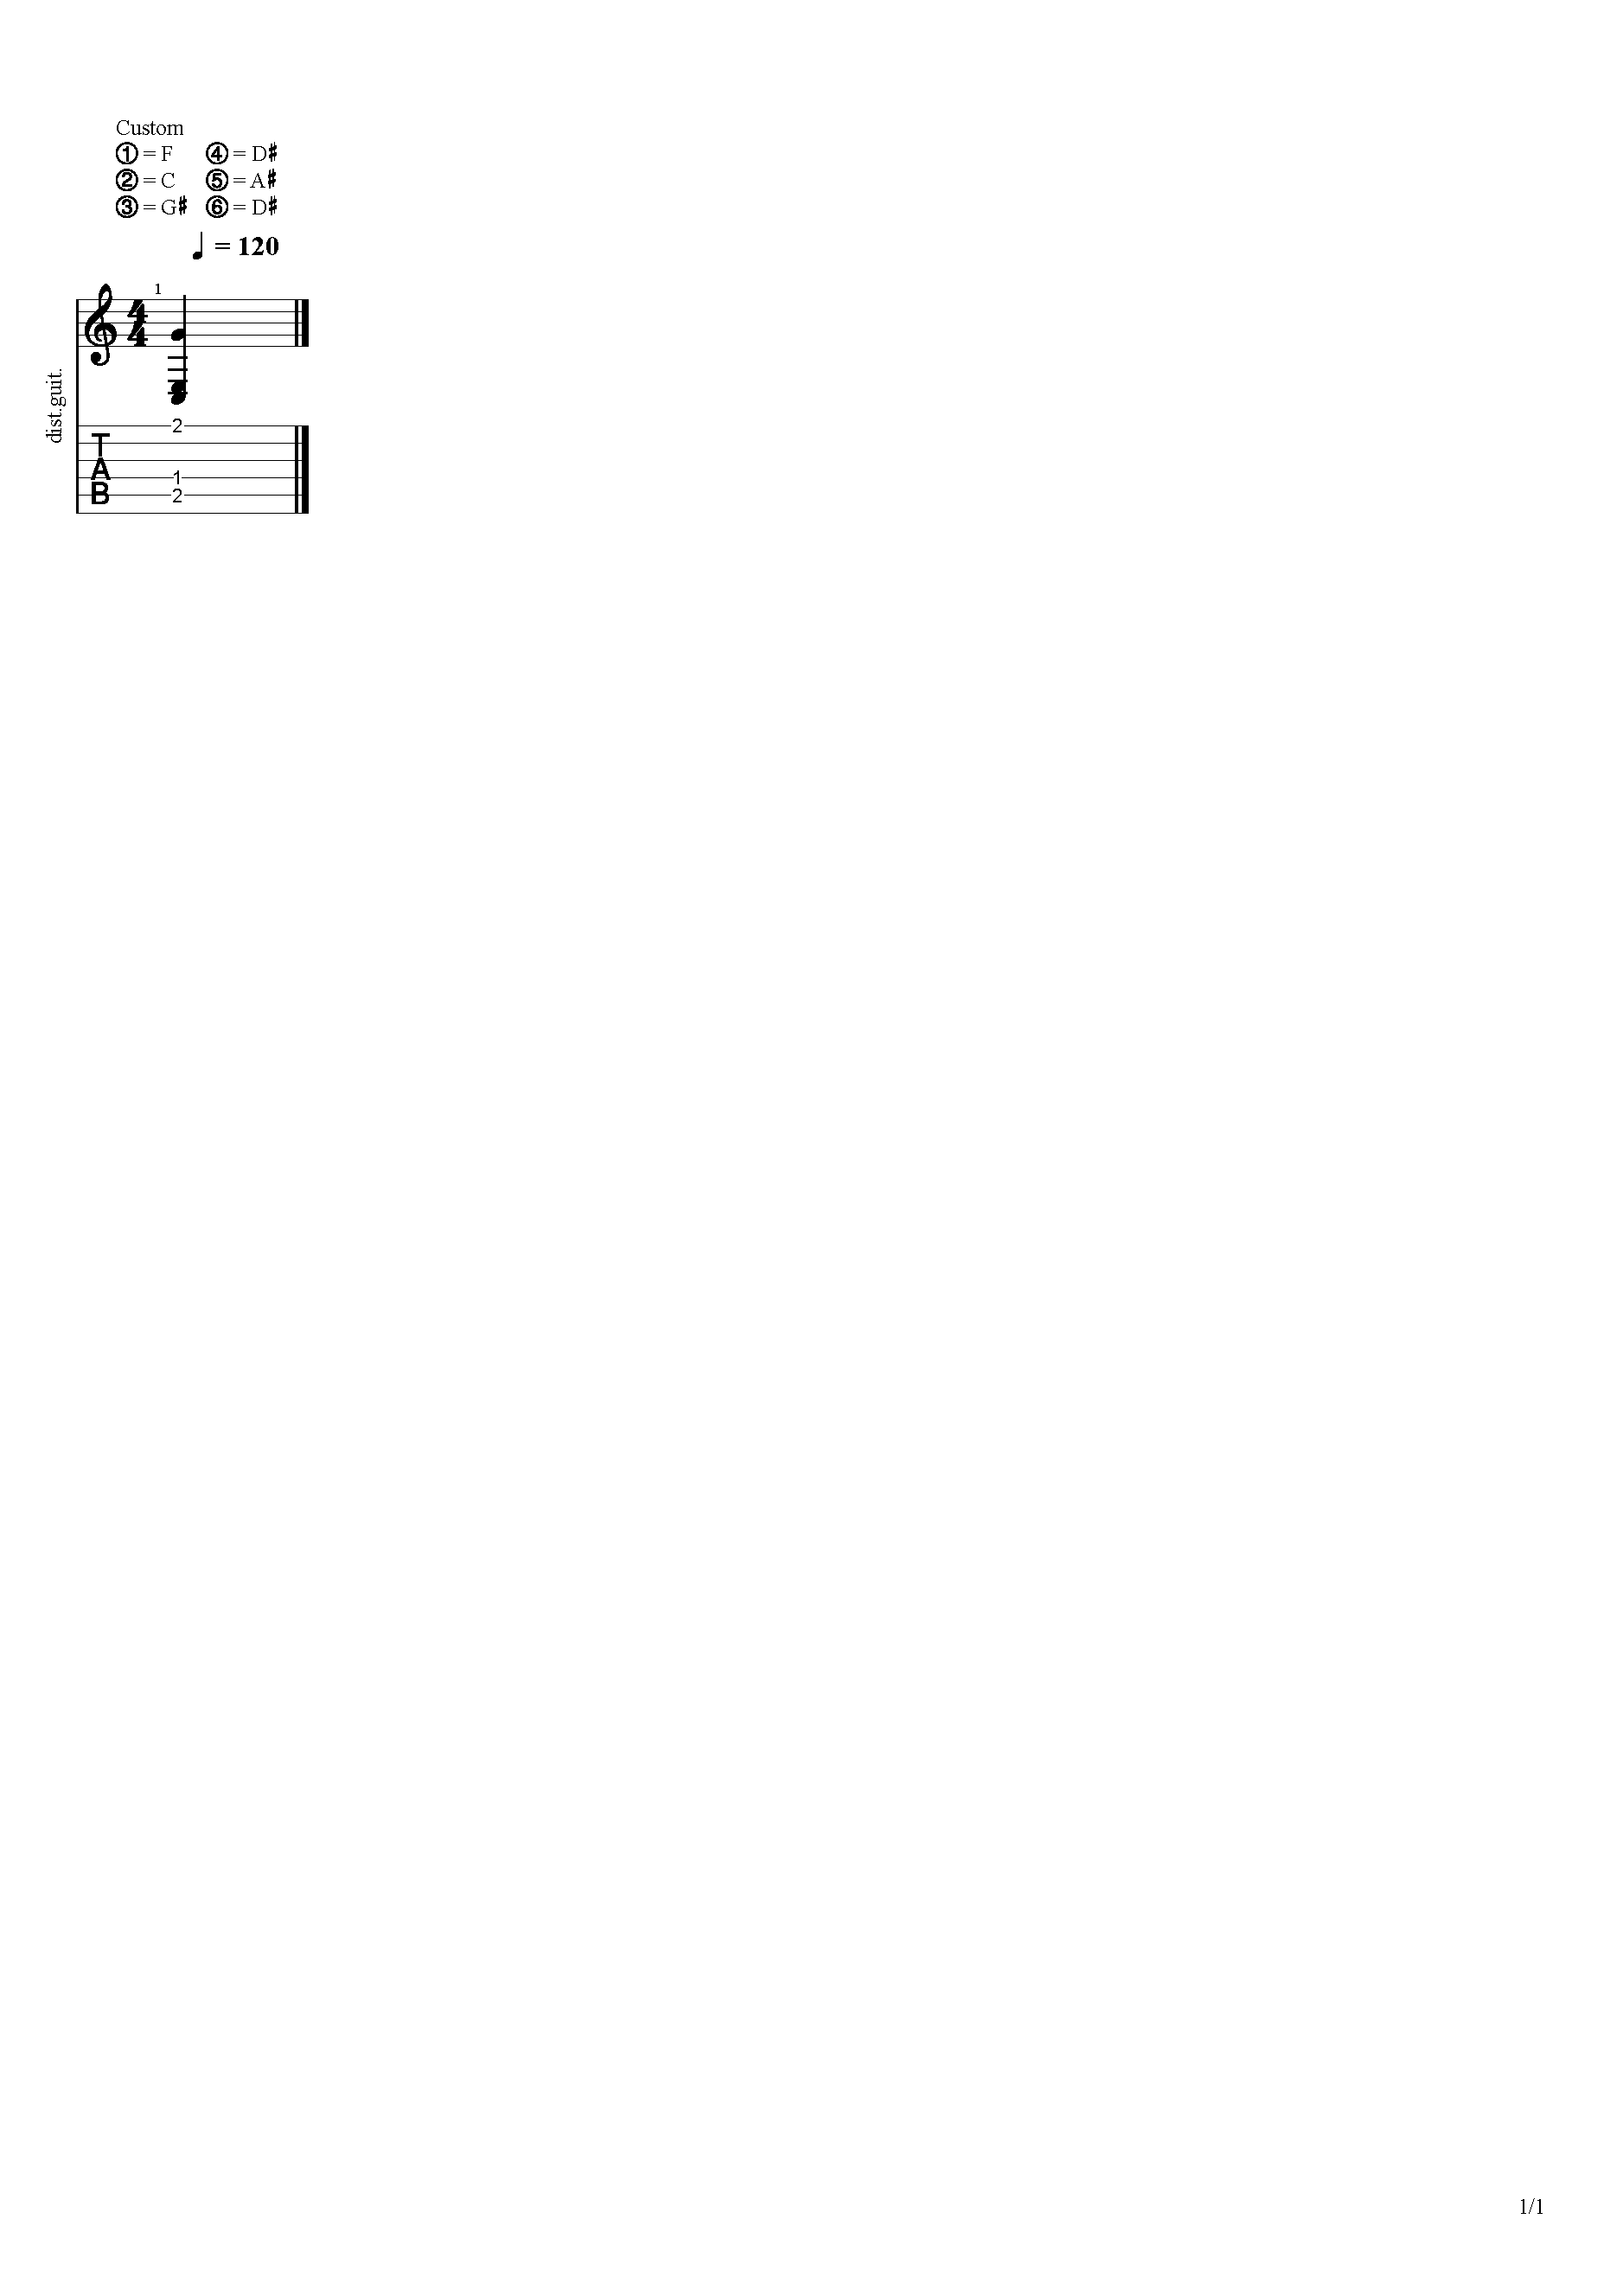
\includegraphics[trim={0 980 650 150}, clip, width=0.7\linewidth]{Cmajor.pdf}
  \caption{C major chord shape on a 6 string. The diagram illustrates muscial notation along with guitar tablature.}
  \label{fig:chord}
\end{minipage}\hfill
\begin{minipage}{0.48\linewidth}
  \centering
  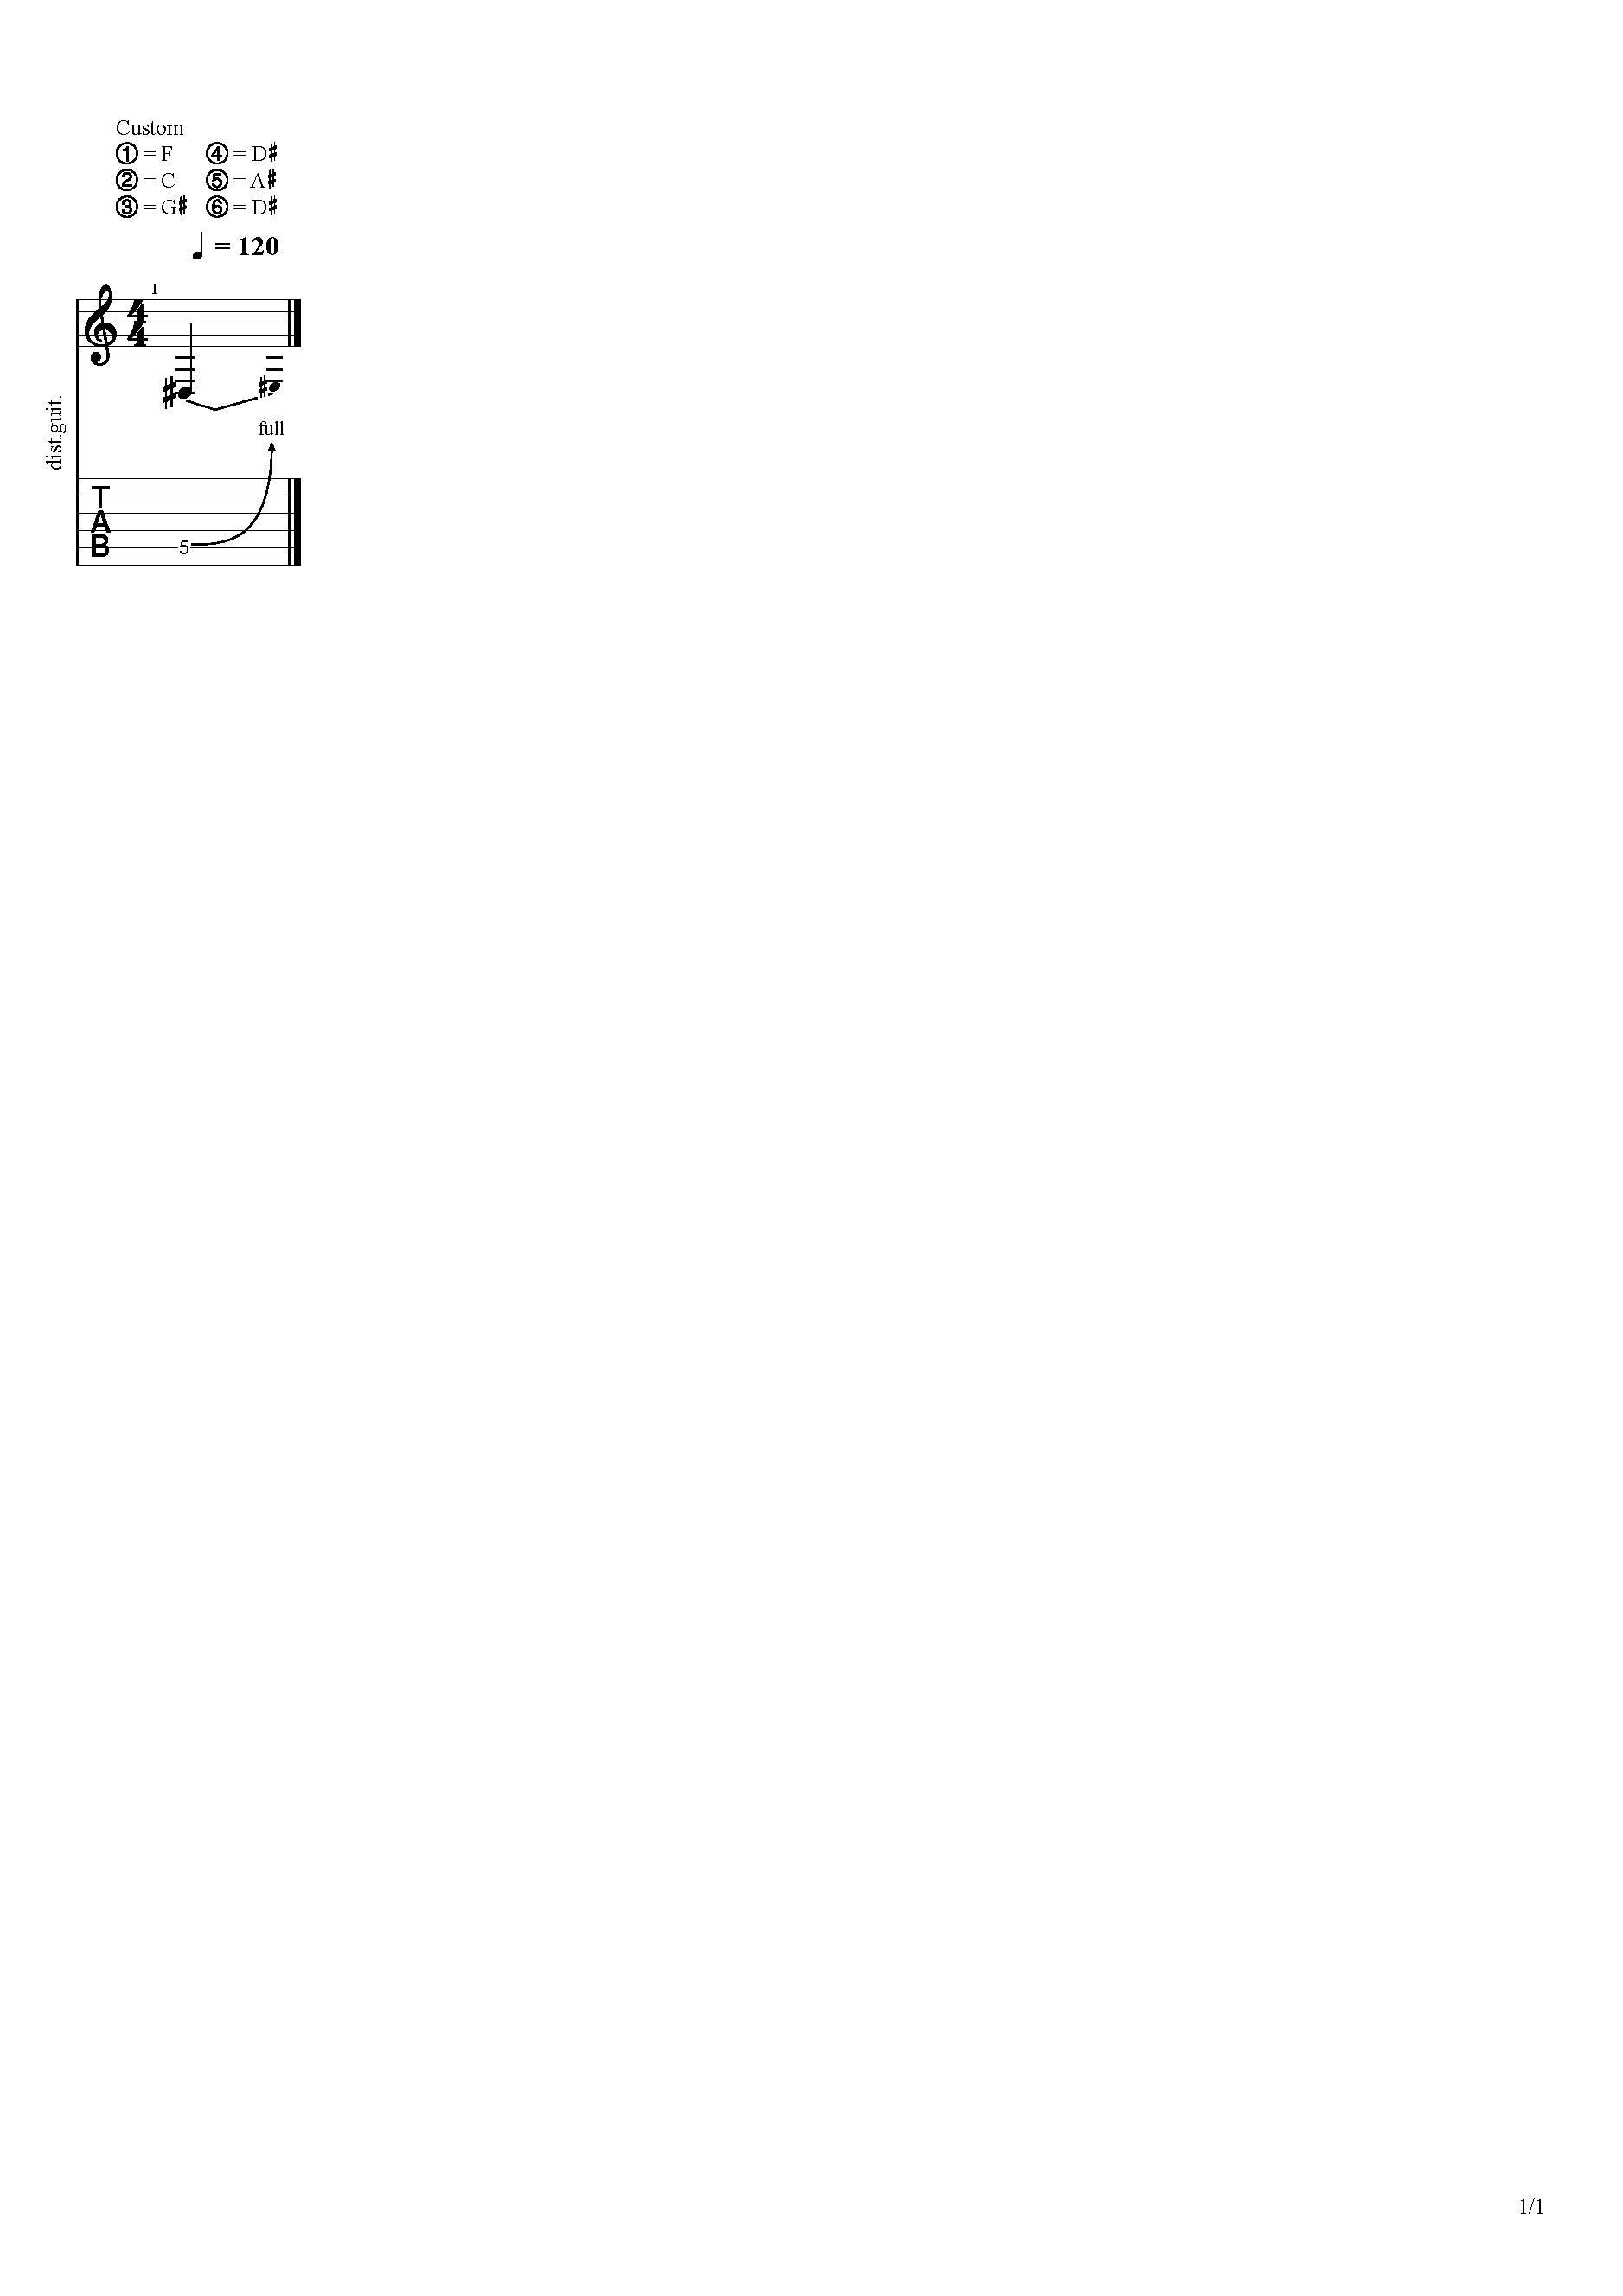
\includegraphics[trim={0 950 650 150}, clip, width=0.7\linewidth]{Note5bend1.pdf}
  \caption{Musical notation and guitar tablature showing full note bend on fret 5, string 5.}
\label{fig:bend}
\end{minipage}
\end{figure}

\subsubsection{Phrases}
A music bar (also called a measure) is a fundamental unit in musical notation that divides
music into segments of equal time, defined by the time signature \citep{Miller2016MusicTheory3E}. Each measure is separated by
a BAR\textsuperscript{~\ref{app:secA1}} token.
\subsection{Embedding}
A bar consists of a fixed number of beats, composed of musical notes that were tokenised as described in Section~\ref{sec:tokenisation}. Each bar is treated like a sentence.
It has been demonstrated that the transformer equipped with relative attention 
is very well-suited for generative modelling of symbolic music \citep{Vaswani2} \citep{zhou2023choir} \citep{li2024hrpe}. 
The chunking strategy used to carry over context between sequences 
during training follows the approach introduced in \citet{chunking}, 
which builds upon Transformer-XL's \citep{transformerXL} segment-level recurrence mechanism. 
This method enables the model to capture longer-range dependencies by 
reusing hidden states from previous token chunks across segments. 
An example of a riff is shown in is given in Figure~\ref{fig:riff}. 
  \begin{figure}[H]
  \centering
  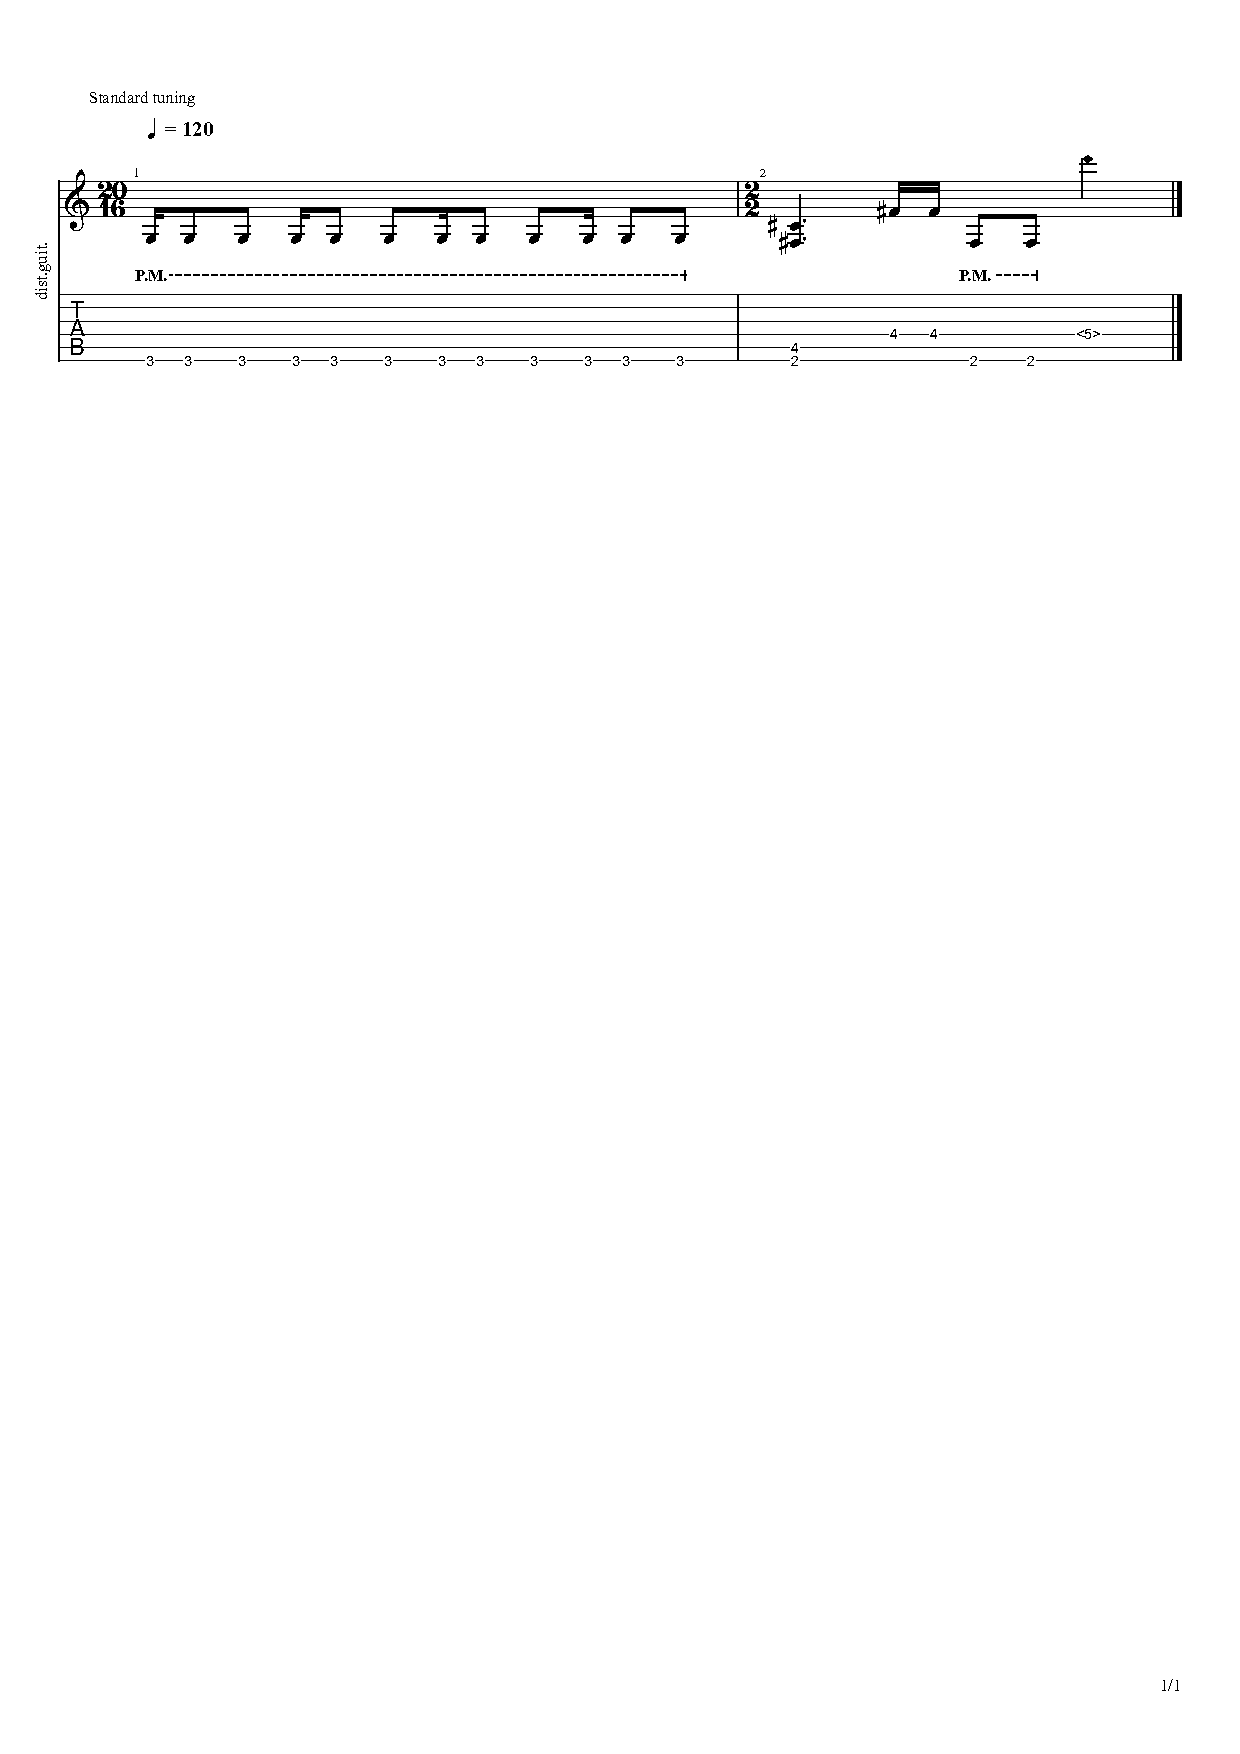
\includegraphics[trim={0 650 0 40}, clip, width=0.8\linewidth]{Riff_example.pdf}
  \caption{Example guitar riff showing a sequence of notes in combination with accents like pinch harmonic, barre chord and palm mute.}
\label{fig:riff}
\end{figure}
An example of 3 sequences with 16 tokens per sequence embedding is as follows: 
\begin{verbatim}
[27049, 7985, 11849, 11849, 7985, 11849, 11849, 7985, 11849,
11849, 7985, 11849, 11849, 27049, 17485, 17506]
[11849, 11849,  7985, 11849, 11849, 27049, 17485, 17506, 27051,
7802, 7802, 11848, 11848, 15530, 27074, 27049]
[27051,  7802,  7802, 11848, 11848, 15530, 27074, 27049, 27075, 0, 
0, 0, 0, 0, 0, 0]
\end{verbatim}
The first two sequences contain musical notes, while the third sequence is padded with zeros to maintain a consistent length of 16 tokens. 
This padding ensures that all input sequences are of uniform length, while still allowing the flexibility to handle variable-length musical phrases.
Overlapping input windows with a fixed stride is generated to increase the number of effective 
training samples and improve context continuity. Such overlapped contexts have been 
shown to increase sample diversity for next token prediction in language modeling tasks \citep{gu-etal-2025-overlapping}, 
and improve segmentation performance \citep{abbasi-etal-2025-neural}.
\subsection{Training}
\subsubsection{Dataset}
The guitar tracks were obtained from \citet{SCORESET}.
The dataset consists of files in .gp5 \citep{GuitarProFormatInfo2025} format in standard tuning. 
From the full set, 6208 sequences were randomly sampled to enable efficient training on standard desktop hardware.
The dataset was split into training, validation, and test sets using the common 80/10/10 ratio \citep{Goodfellow2016DeepLearning}.
For inference, the first 10 notes of each measure from the training set were selected as prompts for sequence generation and evaluation.
Relavant statistics about the dataset used for training and evaluation are provided in \citet{begari2025scoresetdatasetguitarprofiles}.
\begin{figure}[h]
\centering
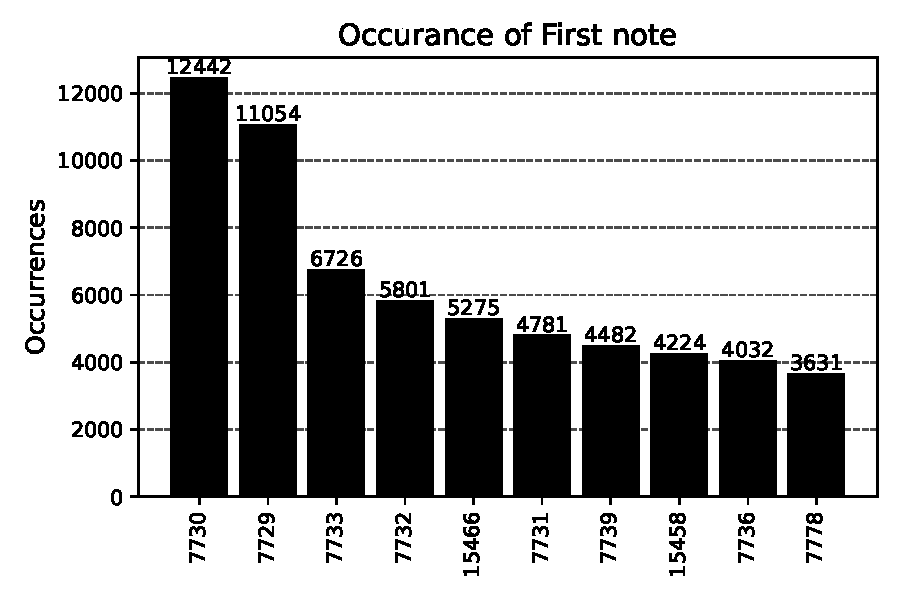
\includegraphics[clip, width=0.5\linewidth]{startprobability.pdf}
\caption{Distribution of starting notes in training data for musical measures, used to select initial tokens at inference time for more consistent generation.}
  \label{fig:firstnote}
\end{figure}

\subsubsection{Model}
The Transformer is built from a decoder-only stack with masked self 
attention as described in \citet{Vaswani2}. Although, segment-level 
recurrence mechanism is captured in Transformer-XL \citep{transformerXL}, 
its memory is limited to one previous segment at a time. To model dependencies across a whole batch, the gaussian distributions of the sequences are learned through a Multi layer Perceptron layer.
If the input is a batch of sequences defined by:
\begin{align}
X \in \mathbb{R}^{B \times T \times d}
\end{align}
where:
\begin{itemize}
    \item \( B \): batch size (number of sequences)
    \item \( T \): number of tokens per sequence
    \item \( d \): embedding dimension
    \item \( X_i \in \mathbb{R}^{T \times d} \): the \(i\)-th sequence in the batch
\end{itemize}

Sequence level mean pooling is performed by:
\begin{align}
\bar{x}_i = \frac{1}{T} \sum_{t=1}^{T} X_{i,t} \quad \in \mathbb{R}^{d}
\end{align}

Gaussian parameters are then computed with a Multi Layer Perceptron.
Let \( f: \mathbb{R}^{d} \rightarrow \mathbb{R}^{2d} \) be a learned MLP.
Then:
\begin{align}
[\mu_i, \log \sigma_i] = f(\bar{x}_i)
\quad \text{with} \quad 
\mu_i, \log \sigma_i \in \mathbb{R}^{d}
\end{align}

Ensure positivity of standard deviation:
\begin{align}
\sigma_i = \exp(\log \sigma_i) + \varepsilon
\quad \text{where } \varepsilon > 0
\end{align}

Each sequence is then represented as a diagonal multivariate Gaussian:
\begin{align}
\mathcal{N}_i = \mathcal{N}(\mu_i, \mathrm{diag}(\sigma_i^2))
\end{align}

The pairwise KL divergence between each pair of Gaussians \citep{kldiv}:
\begin{align}
\label{eq:kldiv}
\text{KL}(\mathcal{N}_i \parallel \mathcal{N}_j) =
\frac{1}{2} \sum_{k=1}^{d} \left[
\log\left( \frac{\sigma_{j,k}^2}{\sigma_{i,k}^2} \right) +
\frac{\sigma_{i,k}^2}{\sigma_{j,k}^2} +
\frac{(\mu_{i,k} - \mu_{j,k})^2}{\sigma_{j,k}^2} - 1
\right]
\end{align}

This produces a KL matrix:
\begin{align}
\text{KL\_matrix} \in \mathbb{R}^{B \times B}, \quad
[\text{KL\_matrix}]_{i,j} = \text{KL}(\mathcal{N}_i \parallel \mathcal{N}_j)
\end{align}

A simpler version of the attention matrix from \citet{XL} is used from which the KL divergence-based sequence bias is subtracted:
\begin{align}
\text{RA}_{\text{KL}} = \text{softmax} \left( \frac{Q K^\top}{\sqrt{d_k}} + Q R^\top - \alpha \cdot \text{KL}_{\text{bias}} \right)
\end{align}
A weighted sum over relative positional value contributions $V_{\text{rel}}$ is then added:
\begin{align}
\text{Output} = \text{RA}_{\text{KL}} \times V + \text{RA}_{\text{KL}} \times V_{\text{rel}}
\end{align}

\subsubsection{Loss}
The model's loss is composed of three components:
\begin{align}
\mathcal{L}_{\text{total}} = \mathcal{L}_{\text{CE}} + \lambda \mathcal{L}_{\text{rep}} + \delta \mathcal{L}_{\text{seq}}
\end{align}
\paragraph{Cross Entropy loss ($\mathcal{L}_{\text{CE}}$)}
Cross-entropy loss is the standard choice for training deep neural 
networks and logistic regression models for both binary and multi-class 
classification tasks \citep{mlglossary}.


\paragraph{Repetition loss ($\mathcal{L}_{\text{rep}}$)} 
Repetition helps organise musical ideas, making pieces more 
coherent and memorable. It gives listeners reference points and expectations, 
aiding in the recognition and recall of themes or motifs \citep{Hu_2022}.
Composers have long used stochastic (probability-based) methods to inject randomness into repeated motifs, 
sometimes even employing quantum randomness for truly unpredictable results \citep{yamada_grandi_munoz-gil_barbiero_aloy_lewenstein_2021}. 
This demands careful consideration, as it relies on the listener's inherent 
ability to recognise patterns and their natural inclination toward novelty. 
Since it is already known that accent tokens\textsuperscript{~\ref{app:secA1}}
cannot repeat, it is penalised through repetition loss, making them less likely to 
be selected again in subsequent steps. 
The concept of the repetition penalty introduced in \citet{reppenalty} uses penalised sampling
at inference time.
The proposed loss is a logits regulizer which is fully differentiable 
and does not require autoregressive sampling
during training, making it compatible with teacher-forced optimization in
decoder-only architectures.
For batch element $b \in \{1,\dots,B\}$ and timestep $t \in \{1,\dots,T\}$, let
$\mathbf{z}_{b,t} \in \mathbb{R}^{V}$ be the output logits of the decoder.

The softmax distribution with temperature $\tau > 0$ is defined as:
\begin{equation}
P_{b,t}(v)
=
\frac{\exp(z_{b,t,v} / \tau)}
{\sum_{u=1}^{V} \exp(z_{b,t,u} / \tau)} ,
\end{equation}
where $v \in \{1,\dots,V\}$.

Let $\mathcal{V}_p \subseteq \{1,\dots,V\}$ denote the set of penalized tokens.
The total probability mass assigned to penalized tokens at timestep $t$ is defined as:
\begin{equation}
S_{b,t}
=
\sum_{v \in \mathcal{V}_p} P_{b,t}(v) .
\end{equation}

The logits-based penalized token adjacency loss is then defined as:
\begin{equation}
\mathcal{L}_{\text{adj}}
=
\frac{1}{B(T-1)}
\sum_{b=1}^{B}
\sum_{t=2}^{T}
S_{b,t-1} \cdot S_{b,t} .
\end{equation}

This loss penalizes the model for assigning high probability mass to penalized tokens
at consecutive timesteps, including both identical token repetition and cross-token
adjacency within $\mathcal{V}_p$.

\paragraph{Sequence loss ($\mathcal{L}_{\text{seq}}$)} 
A sequence memory module is defined that maintains embeddings of sequences. 
Let $N$ denote the number of sequences and $d_{\text{model}}$ the 
embedding dimension. For a sequence ID $i \in \{1, \dots, N\}$, 
the embedding is given by:
\begin{equation}
\mathbf{s}_i = \mathrm{Embedding}(i) \in \mathbb{R}^{d_{\text{model}}}.
\end{equation}
Given hidden states from a transformer model
\[
\mathbf{H} \in \mathbb{R}^{B \times H \times T \times D},
\]
where $B$ is the batch size, $H$ is the number of hidden heads, $T$ the sequence length, and $D$ the hidden dimension per head, hidden states are permuted and flattened as:
\begin{align}
\mathbf{H}_{\text{perm}} &= \mathbf{H}.permute(0, 2, 1, 3) \in \mathbb{R}^{B \times T \times H \times D},\\
\mathbf{H}_{\text{flat}} &= \mathrm{reshape}(\mathbf{H}_{\text{perm}}) \in \mathbb{R}^{B \times T \times (H \cdot D)}.
\end{align}
The sequence-level embedding is then obtained by averaging over time steps and adding the sequence memory embedding:
\begin{equation}
\mathbf{h}_{\text{seq}, i}^{\text{final}} = \frac{1}{T} \sum_{t=1}^{T} \mathbf{H}_{\text{flat}, i, t, :} + \mathbf{s}_i,
\end{equation}
for $i = 1, \dots, B$.
To enforce consistency between the current sequence embedding 
and the learned sequence memory, the mean squared error (MSE) loss is defined as:
\begin{equation}
\mathcal{L}_{\text{seq}} = \lambda \cdot \frac{1}{B} \sum_{i=1}^{B} \left\| \mathbf{h}_{\text{seq}, i}^{\text{final}} - \mathbf{s}_i \right\|_2^2,
\end{equation}

where $\lambda$ is a sequence penalty weight hyperparameter.

This loss encourages the model to maintain a 
representation close to the learned sequence memory, 
improving sequence-level consistency across batches.

\section{Results}\label{sec2}
The idea of context carryover has been well established in \citet{llmgate} \citet{wei2021attentivecontextualcarryovermultiturn} \citet{pmlr-v267-chen25cg}
\citet{rae2019compressivetransformerslongrangesequence} \citet{beltagy2020longformerlongdocumenttransformer} \citet{zaheer2021bigbirdtransformerslonger}. 
During inference, the model carries over context from previous sequences by 
using the last token of the preceding measure as the first token for the 
subsequent measure, following the approach described in \citet{remi}.
To compare the quality of predicted tokens (P)  from true distributions (Q), 
relative entropy is calculated using Kullback-Leibler divergence, following the methodology in
\citet{Seo2016} \citet{zhang2025aestheticshumanpreferencescomparative} \citet{spiliopoulou2011comparingprobabilisticmodelsmelodic}:
\begin{align}
D_{\mathrm{KL}}(P \parallel Q) = \sum_{x \in X} P(x) \log \left( \frac{P(x)}{Q(x)} \right)
\end{align}
\subsection{Grid search}
To determine the optimal configuration, a grid search was performed over a predefined set of hyperparameter values. 
The search included combinations of key parameters such as learning rate, sequence length, model dimensionality, 
Each configuration was trained for 10 epochs, and performance was evaluated on a validation set using loss. 
The best-performing set of hyperparameters was selected based on the lowest validation score.
\begin{figure}[H]
  \centering
  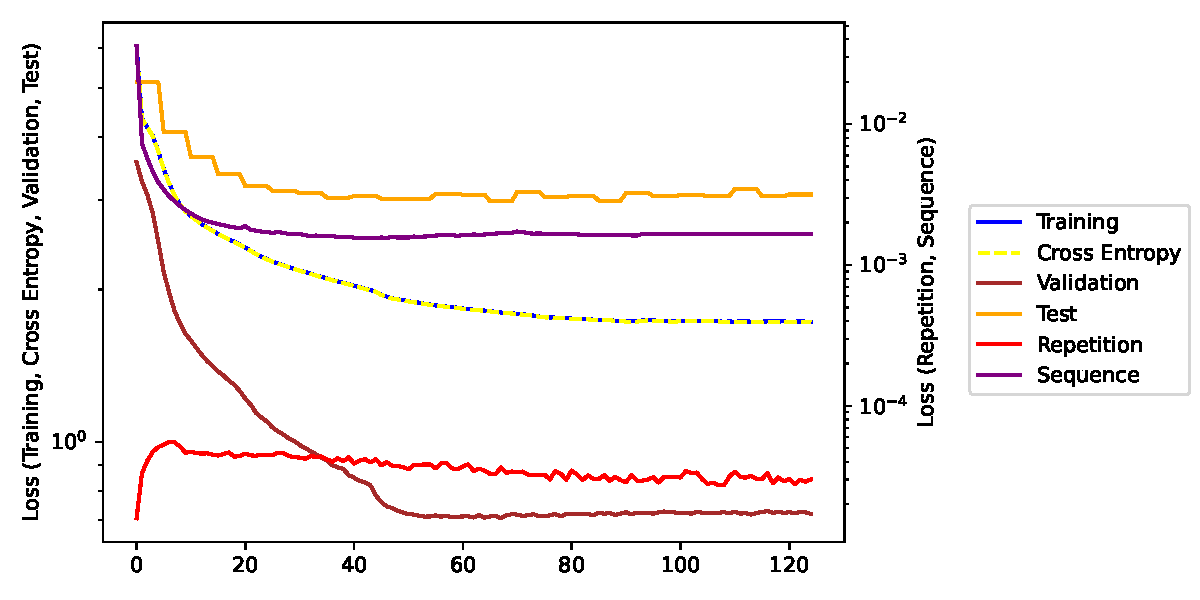
\includegraphics[width=0.8\linewidth]{Loss.pdf}
  \caption{Loss plots over 125 epochs for a median of 3 independent training 
  runs for hyper-parameter values listed in Table~\ref{tab:hyperparam}. Test loss 
  is computed every 5 epochs.}
\label{fig:lossplots}
\end{figure}
\subsection{KL Divergence Evaluation}
To quantitatively assess the model's generative quality, the predicted token distributions were compared with the true distributions using KL divergence.
Figure~\ref{fig:klplots} visualizes the results.
Given that the model is autoregressive and expects an initial token, selecting the start token based on the 
distribution of starting notes of musical measures in the training data yields more consistent generation. The results were averaged over 10 generated phrases per prompt.
\begin{figure}[H]
  \centering
  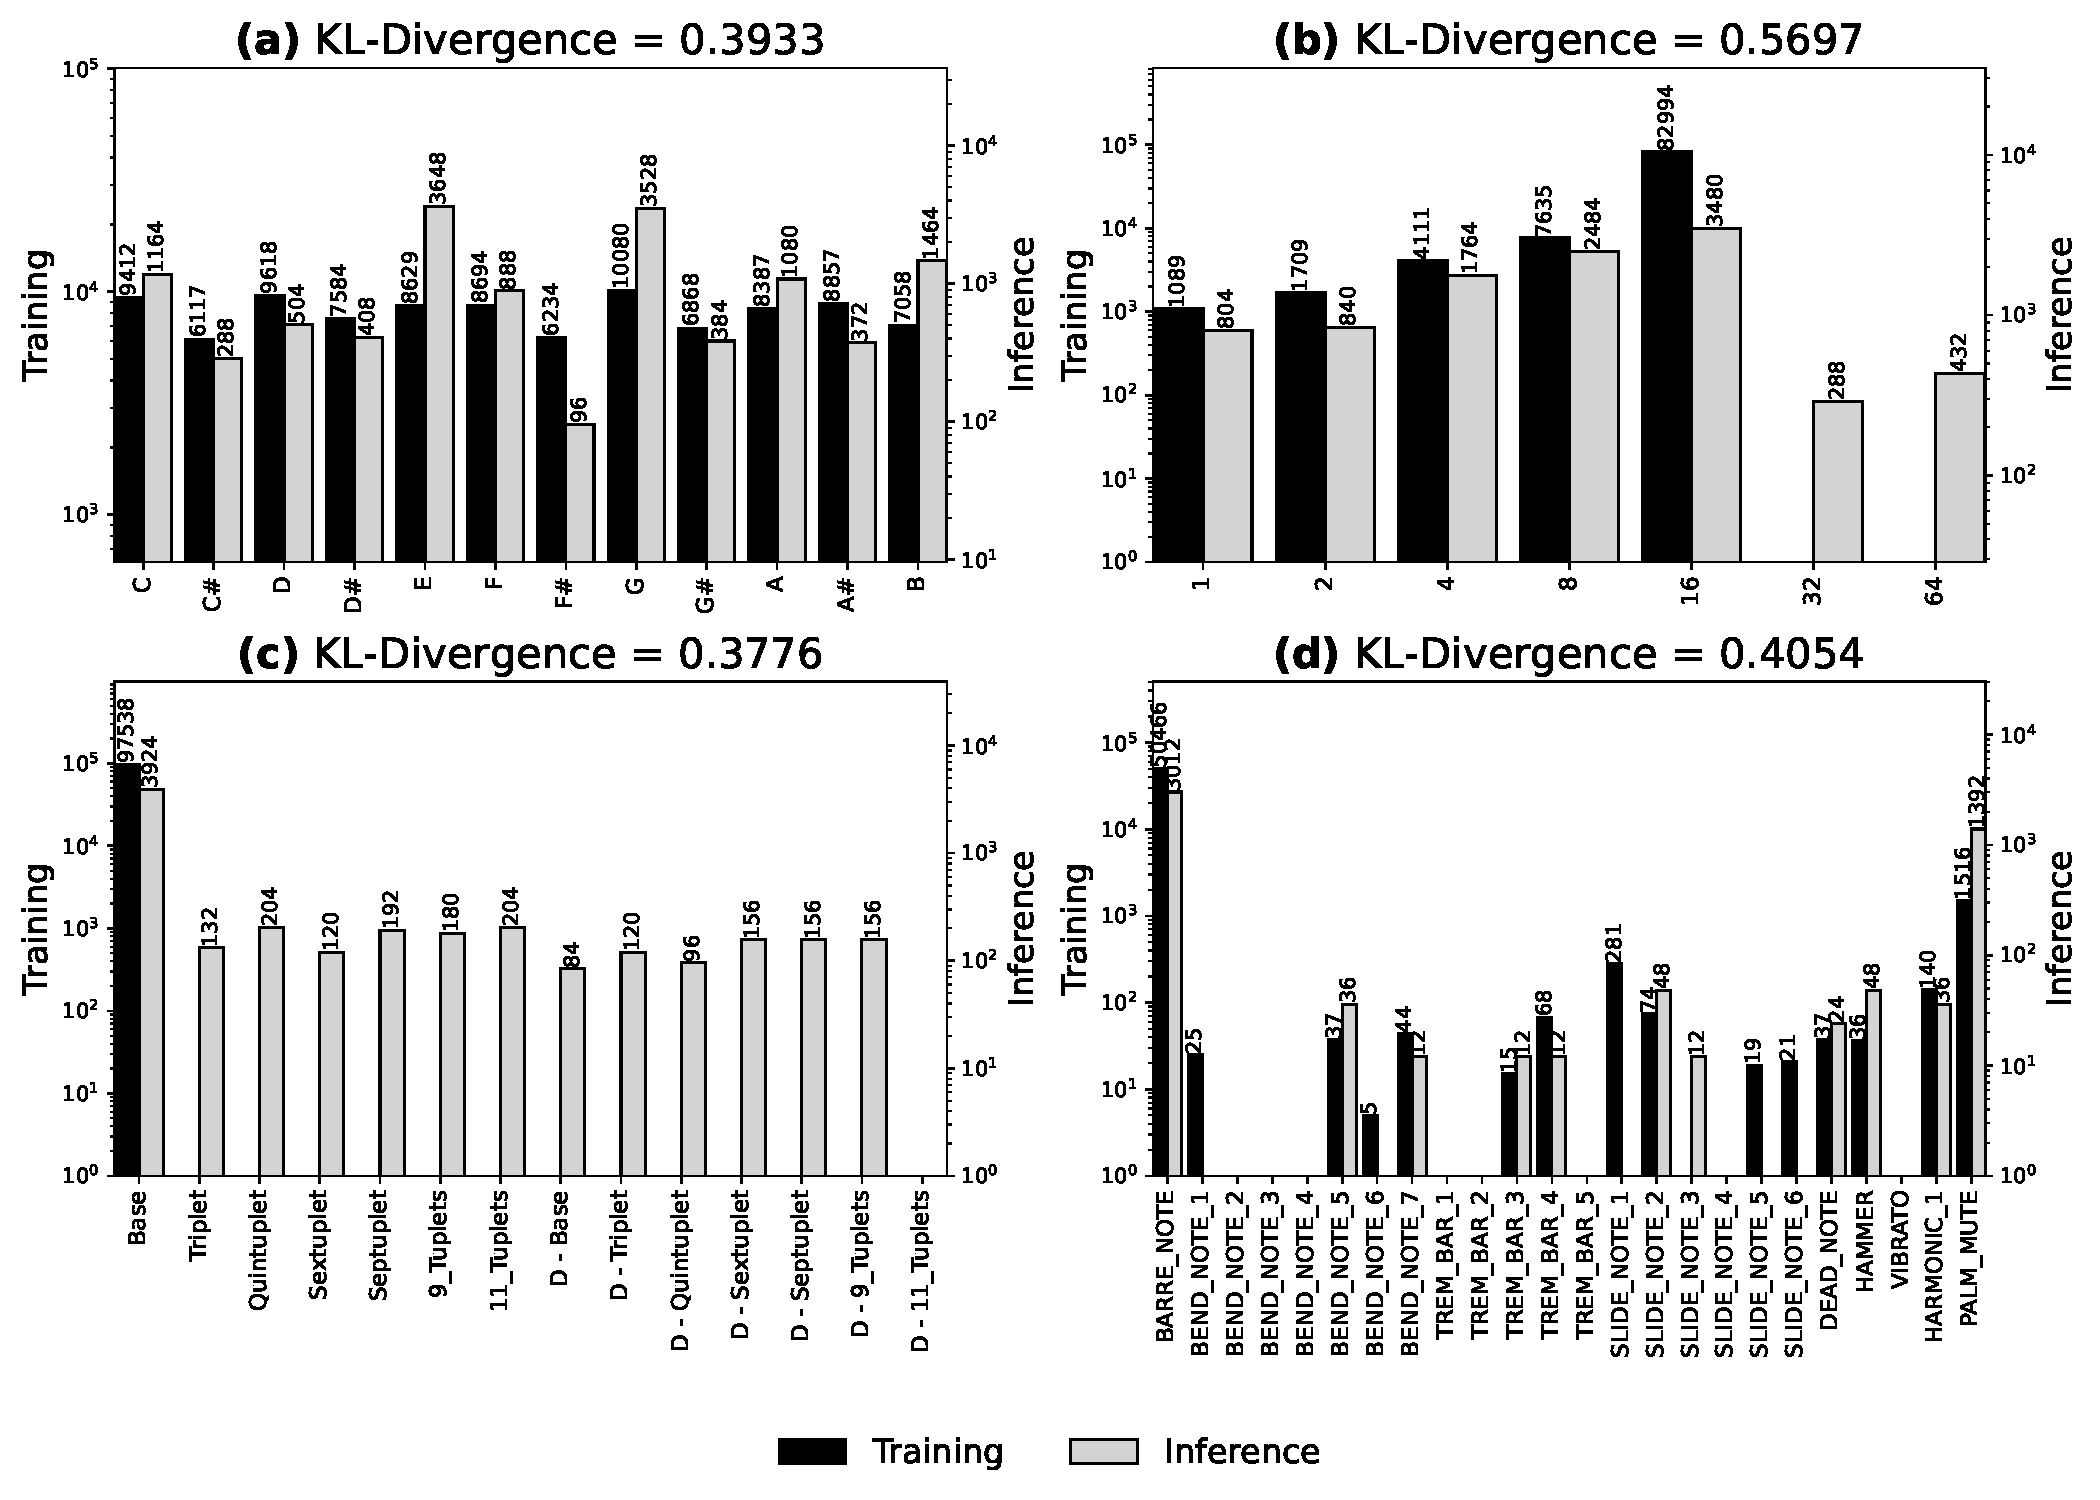
\includegraphics[width=1.0\linewidth]{3_test_all_T_compareprobabilityquad.pdf}
  \caption{KL divergence between inference and training distributions \textbf{(a)} Musical notes, 
  \textbf{(b)} Beats, \textbf{(c)} Beat Types, \textbf{(d)} Accents, indicating prediction by the model.}
\label{fig:klplots}
\end{figure}

\section{Conclusions}\label{sec:conclusions}
The proposed tokenisation scheme efficiently incorporates expressive elements 
without needing an explicit representation like chord vocabulary. The sequence-level attention 
mechanism captures phrase segmentation,
enabling variable-length batching while preserving musical coherence. 
The model demonstrates strong performance in generating guitar riffs with
expressive details, as evidenced by low KL divergence scores across pitch,
beat, and beat type distributions. By incorporating a repetition penalty loss, 
the model naturally reduces redundancy without requiring explicit inference constraints.
Future work could explore extending the
approach to other instruments and incorporating additional musical attributes.
\begin{figure}[H]
  \centering
  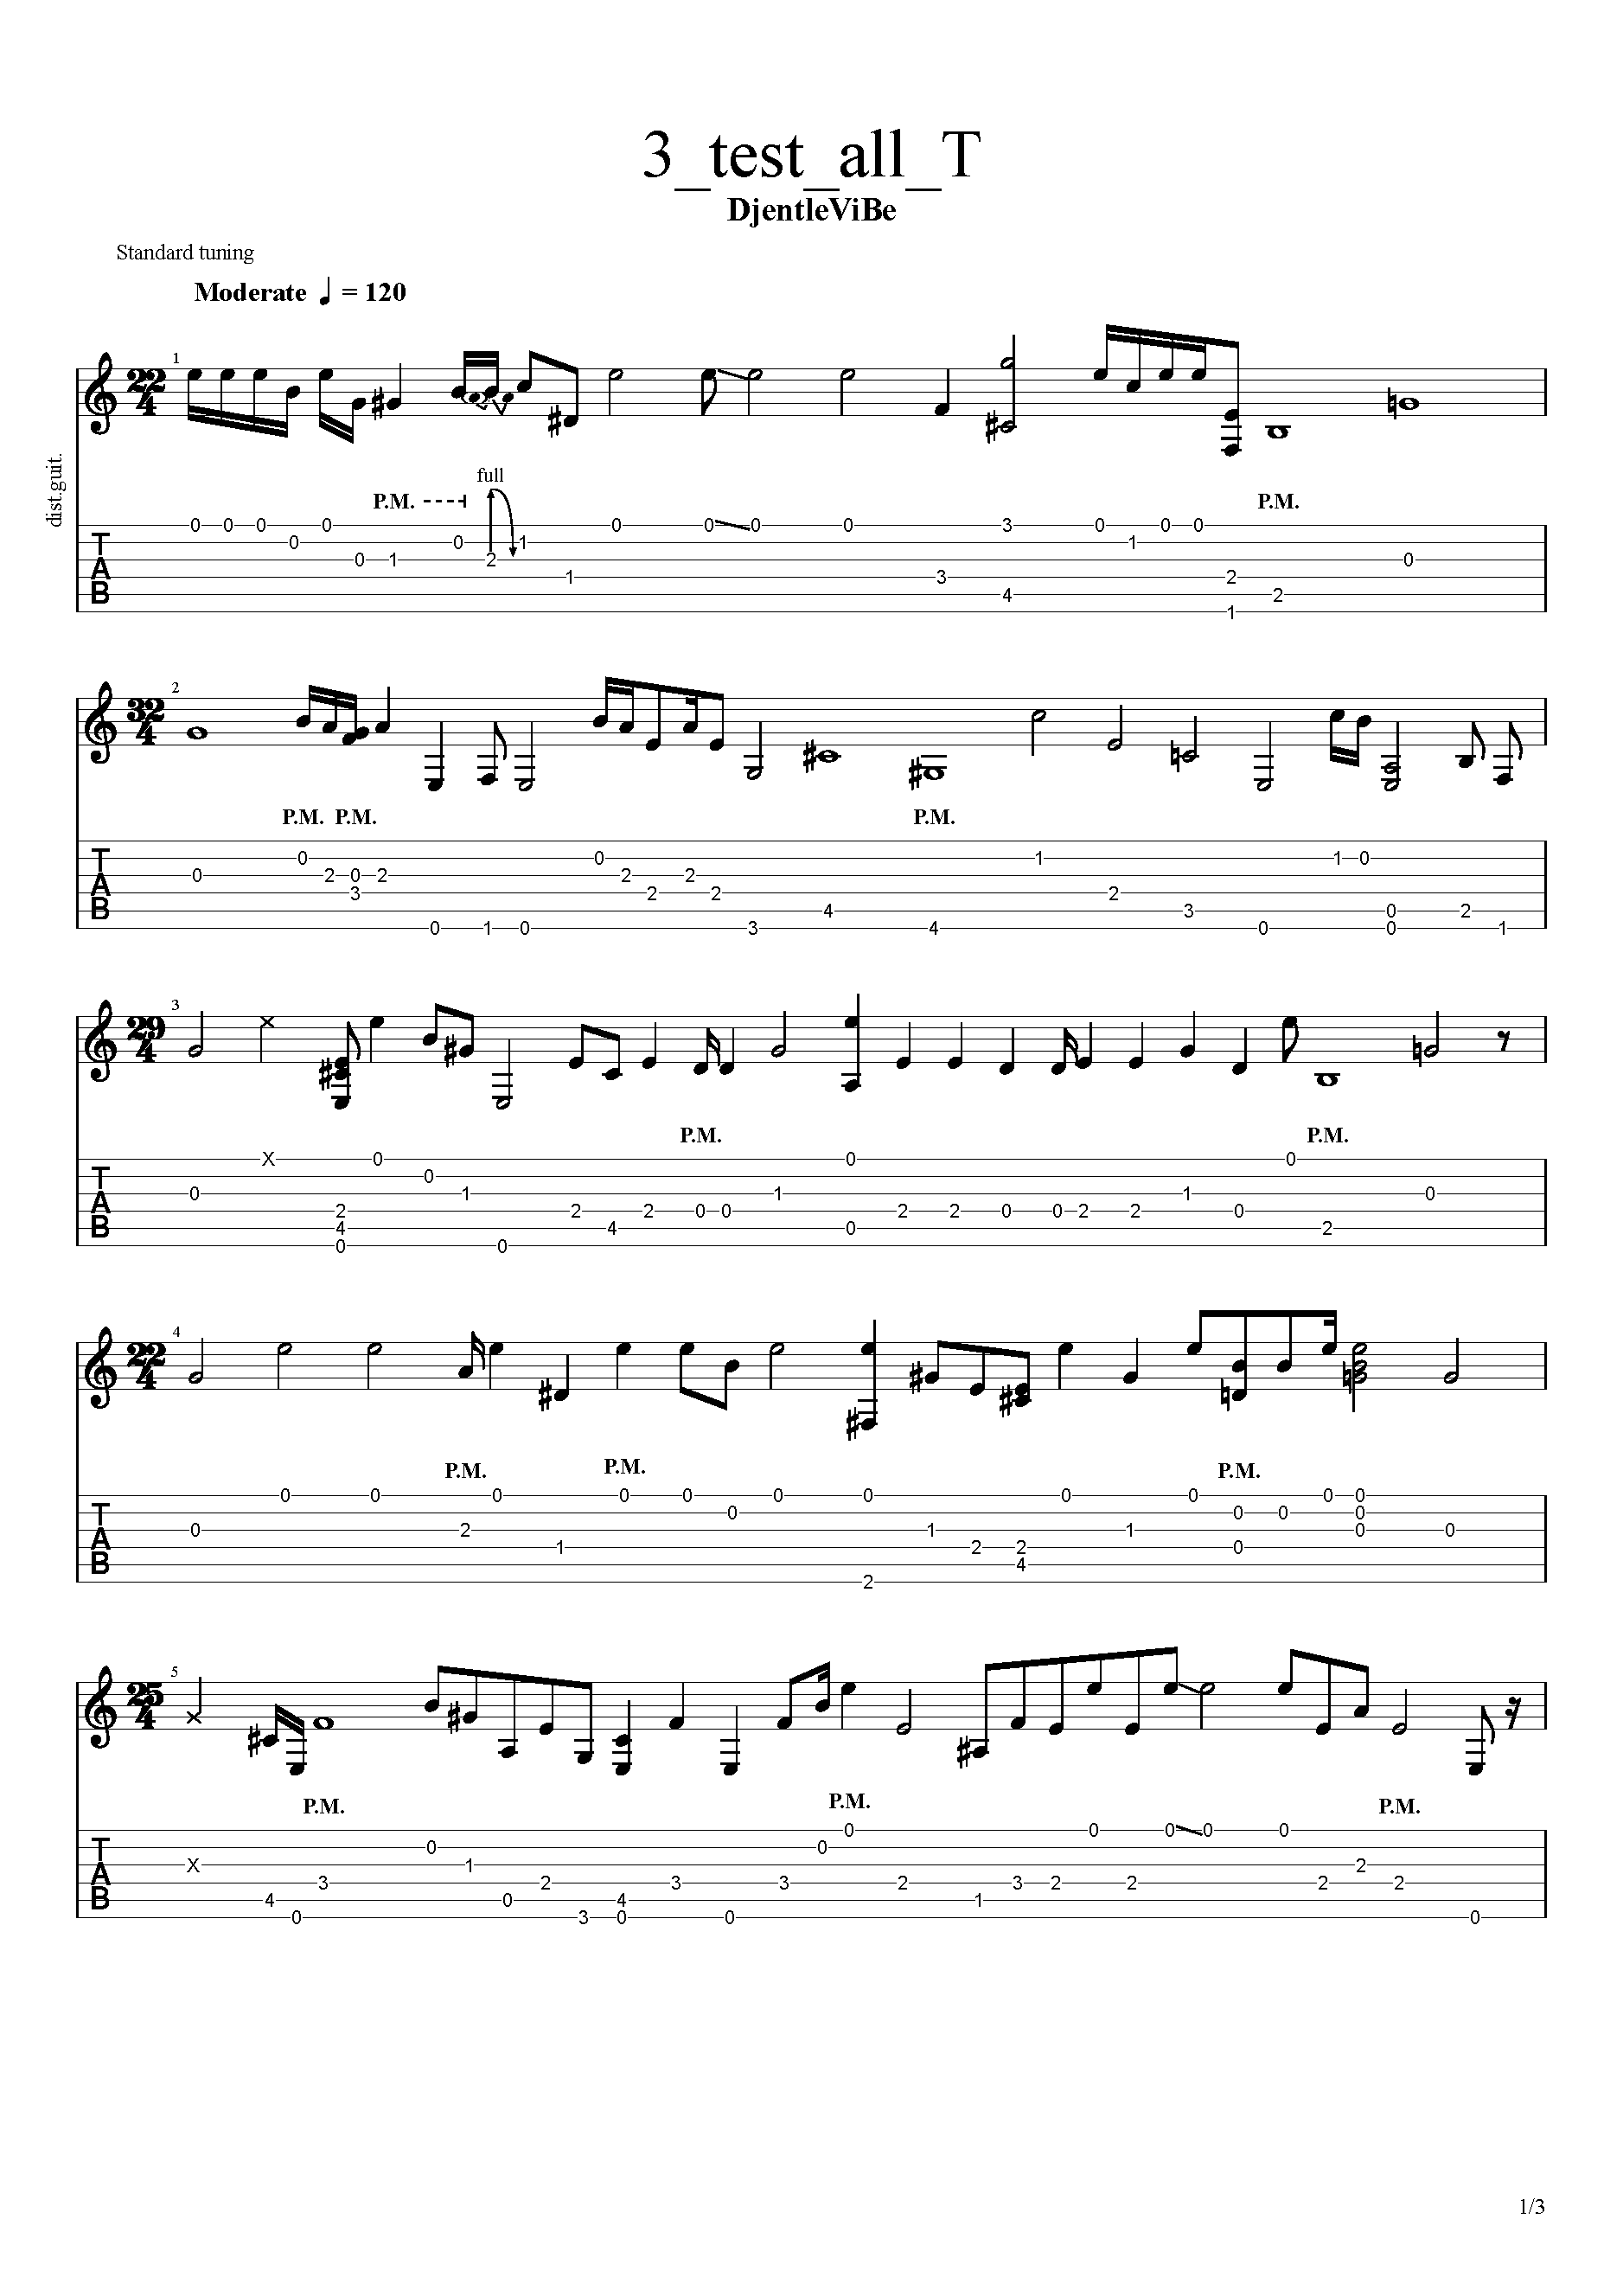
\includegraphics[trim={0 160 0 170}, clip, width=0.9\linewidth]{test_all.pdf}
  \caption{Five generated musical measures demonstrating the model's ability to maintain musical coherence and expressive details at TEMPERATURE 0.7.}
\label{fig:sheet}
\end{figure}
\newpage
\appendix
\section{Token ID}\label{app:secA1}
\begin{table}[!h]
\caption{Token IDs for various accents.}
\label{tab:k}
\begin{center}
  \begin{tabular}{ll}
  \bfseries Accent & \bfseries Token ID
  \\ \hline \\
BAR  & 27049\\
BOS  & 27050\\
BARRE\_NOTE & 27051\\
BEND\_NOTE\_1 & 27052\\
BEND\_NOTE\_2 & 27053\\
BEND\_NOTE\_3 & 27054\\
BEND\_NOTE\_4 & 27055\\
BEND\_NOTE\_5 & 27056\\
BEND\_NOTE\_6 & 27057\\
BEND\_NOTE\_7 & 27058\\
TREM\_BAR\_1 & 27059\\
TREM\_BAR\_2 & 27060\\
TREM\_BAR\_3 & 27061\\
TREM\_BAR\_4 & 27062\\
TREM\_BAR\_5 & 27063\\
DEAD\_NOTE & 27064\\
SLIDE\_NOTE\_1 & 27065\\
SLIDE\_NOTE\_2 & 27066\\
SLIDE\_NOTE\_3 & 27068\\
SLIDE\_NOTE\_4 & 27069\\
SLIDE\_NOTE\_5 & 27070\\
SLIDE\_NOTE\_6 & 27071\\
HAMMER & 27072\\
VIBRATO & 27073\\
HARMONIC\_1 & 27074\\
EOS  & 27075\\
  \end{tabular}
\end{center}
\end{table}
 \section{Hyper-parameter tuning}\label{app:secA2}
The following hyper-parameter values were used for training the model:
  \begin{table}[h]
  \caption{Hyper-parameter values used for training.}
\label{tab:hyperparam}
\begin{center}
  \begin{tabular}{ll}
  \bfseries Property & \bfseries Value
    \\ \hline \\
FFN\_HIDDEN  & 1024 \\
MAX\_SEQ\_LENGTH & 32 \\
NUM\_HEADS & 4 \\
DROP\_PROB & 0.3 \\
NUM\_LAYERS  & 2 \\
D\_MODEL & 256 \\
TEMPERATURE  & 1.0 \\
OVERLAP & 8 \\
LAMBDA & 1.5 \\
ALPHA & 0.1 \\
DELTA  & 1.0 \\
  \end{tabular}
\end{center}
\end{table}
The values were obtained after performing a grid search for 10 epochs and selecting values which gave the lowest validation loss. 
The ranges for the grid search are given in the repository \url{https://github.com/DjentleViBe/SCORE}.
\subsubsection*{Acknowledgments}
This research received no specific grant from any funding agency in the public, commercial,
or not-for-profit sectors.

\bibliography{iclr2026_conference}
\bibliographystyle{iclr2026_conference}

\end{document}
